% Chapter Template

\chapter{A Work Sharing System} % Main chapter title

\label{Chapter3} % Change X to a consecutive number; for referencing this chapter elsewhere, use \ref{ChapterX}

\lhead{Chapter 3. \emph{Apache SparkSQL}} % Change X to a consecutive number; this is for the header on each page - perhaps a shortened title

%----------------------------------------------------------------------------------------
%	SECTION 1
%----------------------------------------------------------------------------------------

\section{Work Sharing}

In large data ware houses, many queries are usually submitted at the same time by multiple users. In the context of big data, a query would take long time to run. There are some data that would be used more frequently than the others, so we can avoid the redundant computations by sharing works among those queries and reduce the total amount of execution time. \\
The idea of work sharing originally comes from Multiple Query Optimization (MQO) \cite{sellis1988}. There are many works on traditional database systems \cite{cosar1993} \cite{bayir2007} \cite{georgios2012} \cite{stavros2005} and also on Hadoop MapReduce have been published. Olston et al. worked on a system called CoScan \cite{olston2011}, a system for sharing data and processing costs among multi-step MapReduce workflows which are executed in Hadoop. In Apache Pig, a number of work sharing optimizations \cite{pigmqo} have been used with the idea of MQO. The current state-of-the-art work in this field is MRShare\cite{nikiel2010} on Apache Hadoop. With the grouping technique, it provides the map input sharing to share scan of input files and map output sharing for saving cost of communication.\\
%----------------------------------------------------------------------------------------
%	SECTION 2
%----------------------------------------------------------------------------------------

\section{SparkSQL Server}
All the works above are only supported for Hadoop MapReduce and they are focused only on a part of work sharing, then they are hard to extend when users want to have new sharing techniques. To the best of our knowledge, there is no published work about Multi Query Optimization on Apache Spark. In our work, we present a new system called SparkSQL Server, which is focused on work sharing among multiple queries.\\

SparkSQL Server is an open source project and hosted at our team's Github.

SparkSQL Server supports queries written in SQL by using DataFrame API of SparkSQL or in produceral languague supported by SparkCore itself.\\

The system does not only care about work sharing among multiple queries but also the scheduling mechanisms to associate with the sharing techniques or to fullfil the users' requirements.\\

The system is generalized so it can support many types work sharing. All the modules of SparkSQL Server are easy to extend, this lets users and developers easily plug their own implementations into the system.\\

\subsection{System Design}
\begin{figure}
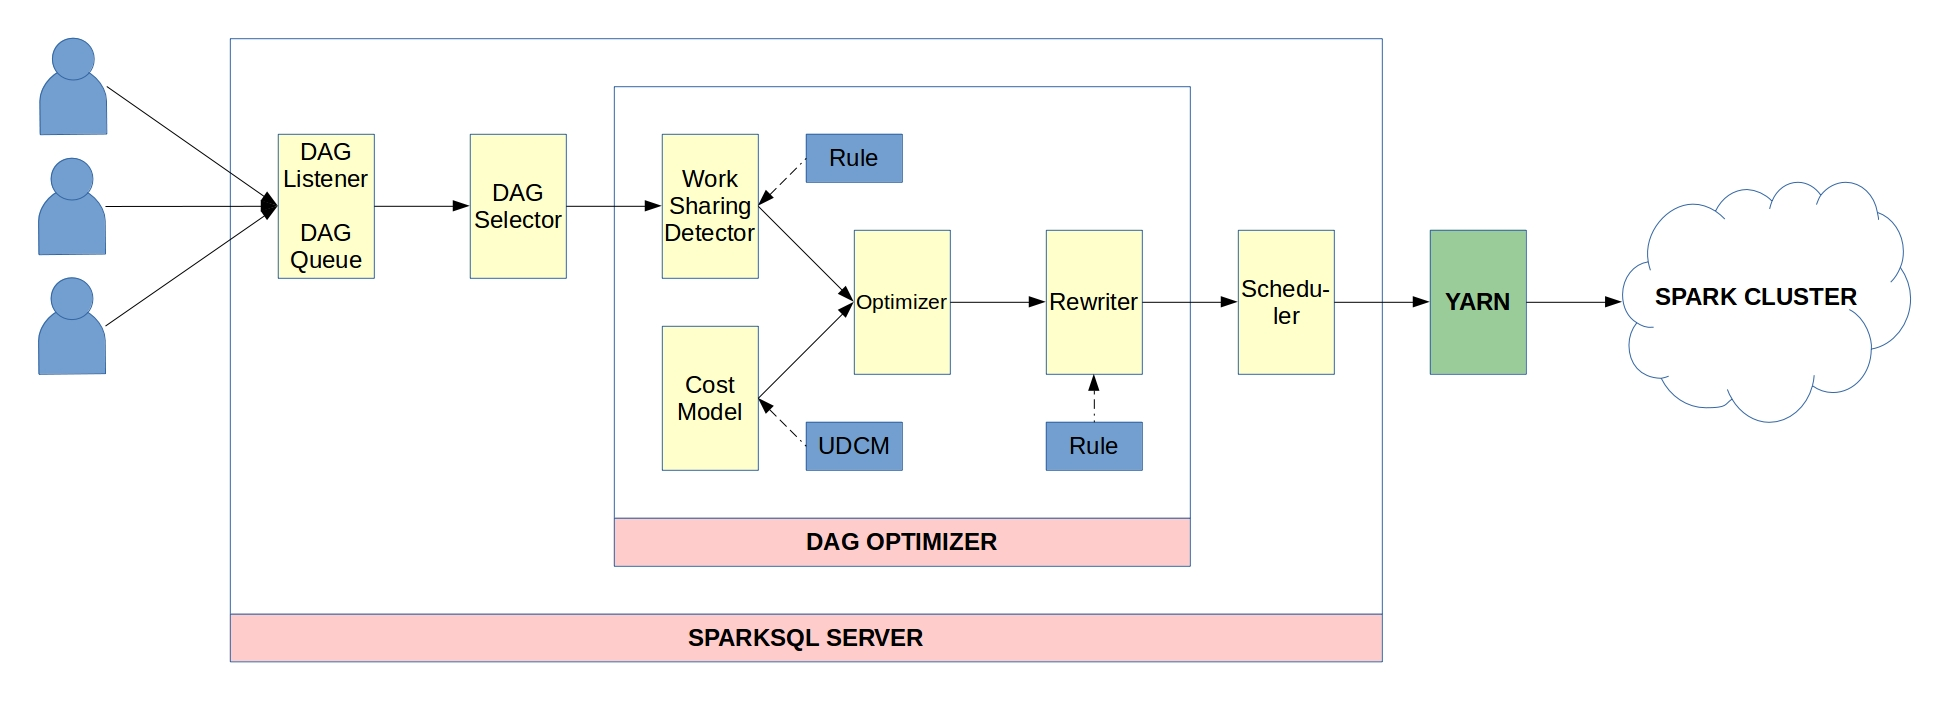
\includegraphics[width=\textwidth]{Figures/sparksql-server-design.jpg}
\caption{The design of SparkSQL Server}
\label{fig:sparksql-design}
\end{figure}
The design of our system aims at the generalization and extensibility so users and developers can easily plug their own implementations. Figure \ref{fig:sparksql-design} expresses the design of our system.\\

Overall, our system has two sides: client side and server side.\\
\textbf{Client side} The client submits the query and needed information to SparkSQL Server so SparkSQL Server can reconstruct exactly the query happened at client side. The query can be written by using produceral operations in Spark or relational operations in SparkSQL or the combination of both types of operations.\\
\textbf{Server side}  The SparkSQL Server contains three main components:\\
\begin{itemize}
\item The Listeners, which listen for client connections and communicate with them.
\item The DAG Optimizer is the heart of our system. All the detections, optimizations, and transformations happen here. The DAG Optimizer is composed of:
\begin{itemize}
\item WorkSharing Detector: this module detects the sharing opportunities among a batch of jobs which has just received from clients. The detector uses rule-based mechanism to detect the sharable jobs. Users can easily write their own rules to detect sharable jobs with many types of sharing.
\item CostModel: it calculates the cost of each execution plan. Users provide their own cost model by the User-defined Cost Model.
\item Optimizer: it receives the input from the output of WorkSharing Detector and uses the CostModel to pick the best DAG or set of DAGs to execute.
\item Rewriter: the Rewriter transforms the original execution plans into the optimized execution plans and then submits them to the Schedulers. The transformation is also based on the rule-based mechanism. It is very easy to define a new rule to support another type of sharing.
\end{itemize} 
Again, all of these four modules are extendable so users can plug their owns into these modules.
\item The Schedulers, which are used to fulfill users' requirements and to associate with the sharing techniques. These Schedulers are aslo extensible so users can plug their own shechuling strategies.
\end{itemize}

\subsection{Implementations}
Similar to the above subsection, we present the implementation of our system on both client side and server side. The order of the explaination is the same as the flow in figure \ref{fig:sparksql-design}.\\
\textbf{Client side} We modify the spark-submit command so that it does not send the application to the cluster manager but to the SparkSQL Server, using this option:  --sparksql-server\\
Each client starts it own driver with its own SparkContext. Then, the client can generate its DAG, the DataFrame creation and send those information: DAG, DataFrame generation, SQL Query to the SparkSQL Server.\\
The client needs to send the jar file, because it contains all user defined functions, classes which are very important to reassemble the DAG at server side. It also needs to send needed information so the SparkSQL Server can reconstruct the DAG and the query. Don’t forget that the query has already been optimized by Catalyst at the client side.\\
\textbf{Server side}
\begin{itemize}
\item \textbf{DAG Listener and DAG Queue} DAG Listener accepts the clients’ connections and receives DAGs, queries and other information they send. Then, it passes to the DAG Queue, the DAG Queue accepts the information the clients send at the FIFO order. In this component, the full DAG of each user will be built based on the initial DAG, the DataFrame creation information and the query. The DAG Queue has a window with fixed size, after reaching the size of the windows, DAG Queue will send a batch of DAGs (and queries also) into the next components. The window size right now is fixed as a constant, it will be changed when we take care of scheduling.
\item \textbf{DAG Selector} This component is something called a pre-scheduler, which will based on the constraint attached with each query to fulfill user’s requirements. For example: job submitted with a deadline. Right now, it just uses the simple FIFO strategy.
\item \textbf{Worksharing Detector} This component will detect which DAGs have the opportunity for worksharing, which DAGs haven’t. Remember that worksharing here is not only sharing scan, it can also have other variants such as sharing group-by or join. It works as rule-based mechanism to detect the worksharing opportunity. The Worksharing Detector bases on the associated rule to find which DAGs have the common part that can be shared. For example, with scan sharing rule, since we always have a pattern of a DAG is that when reading a file from disk, it always contains the HadoopRDD with the attached inputfile path, the rule tries to find each inputfile path of each DAG and puts into an array, then it intersects all the arrays to find out which DAG is shareable.
\item \textbf{Cost Model} It provides an interface so that users can plug their own cost model, which is called User defined cost model, into the system. We can have many types of Cost Model. The cost model can give score, which is calculated from functions, on each DAG or on a batch of DAG.
\item \textbf{Optimizer} With a bag from the output of the previous and a cost model associated with its sharing type, the Optimizer component will do the job: pick the plan with the lowest cost. The Optimizer and the CostModel work closely to find out the best result. For example, the Optimizer can generate many combinations of shareable DAGs and give them to the CostModel, the CostModel evaluates them with scores and gives back to the Optimizer. The Optimizer then choose the combination with the best score.
\item \textbf{Rewriter} This component has many families of rewrite. Each family will have many rewrite rules. It will generate a rewritten DAG which can be optimized, and use the rule that Optimizer picked to transform the original DAGs into the new ones. Each sharing technique can have one or more than one rewriter rules. For example, with sharing scan, we can have the rewrite technique using MRShare or caching.
\end{itemize}


There are some special data structures to wrap a DAG after going through a component:\\
\begin{itemize}
\item DAGContainer: use to wrap a DAG when it is received at DAGListener. It contains a DAG and metadata that it brings together.
\item AnalysedBag: use to wrap an array of DAGContainers after it went through the WorkSharing Detector. It contains an Array of sharable DAGContainer. It also contains a label to indicate which type of sharing it is since there are many types of sharing.
\item OptimizedBag: use to wrap an array of DAGContainers after it went through the Optimizer. It  contains an array of DAGContainers, which is the best combination of DAG after going through the Optimizer. It also contains a label to indicate its sharing type and the Rewritten Rule to indicate which rule it will use to rewrite. A no-sharable DAG is also wrapped into an OptimizedBag with the Rewritten Rule equals to Null.
\item RewrittenBag: use to wrap a rewritten OptimizedBag after the optimized bag went through the Rewriter.
\end{itemize}


\subsection{An Example on SparkSQL Server}

This section gives us an example of SparkSQL Server in action so we can understand how SparkSQL Server works clearly.
Three examples below are similar to the example in section 2.2.3 and we focus only on scan sharing in this example. We also use the MRShare technique, which will be described in details in next chapter, for the Optimizer and Rewriter. The explaination has three parts for each components: Input, Output, and we relate them to the example.\\
\textbf{User1}

\begin{lstlisting}
case class Teacher(name: String, age: Integer)
val input = sc.textFile("hdfs://A.txt")
val people = input.map(_.split(",")).map(p => Teacher(p(0), p(1).trim.toInt))
val peopleDF = people.toDF()
peopleDF.registerTempTable("people")
val teacher = sqlContext.sql("SELECT name FROM people WHERE age <= 50")
val result = teacher.map(t => "Name: " + t(0)).collect.foreach(println)
\end{lstlisting}

\textbf{User2}

\begin{lstlisting}
case class Student(fullname: String, age: Integer)
val input = sc.textFile("hdfs://A.txt")
val people = input.map(_.split(",")).map(p => Student(p(0), p(1).trim.toInt))
val peopleDF = people.toDF()
peopleDF.registerTempTable("people")
val student = sqlContext.sql("SELECT name FROM people WHERE age >= 19")
val result = student.map(t => "Name: " + t(0)).collect.foreach(println)
\end{lstlisting}

\textbf{User3}

\begin{lstlisting}
case class Person(name: String, age: Integer)
val input = sc.textFile("hdfs://B.txt")
val people = input.map(_.split(",")).map(p => Persion(p(0), p(1).trim.toInt))
val peopleDF = people.toDF()
peopleDF.registerTempTable("people")
val adults = sqlContext.sql("SELECT name FROM people WHERE age >= 25")
val result = adults.map(t => "Name: " + t(0)).collect.foreach(println)
\end{lstlisting}

\textbf{Client Side}
\begin{itemize}
\item Input: Users’ applications (jar files)
\item Output: Jarfile, DAGs, DataFrame creation information, SQL queries, mapOutputRatio (the ratio between map output size and input file size) for MRShare are sent to SparkSQL Server. In those example, we have DAG1, DAG2, DAG3.
\end{itemize}

\textbf{Server Side}\\
\textbf{DAG Listener and DAG Queue}
\begin{itemize}
\item Input: DAGs and queries from clients
\item Output: Array of DAGContainers, the metadata is updated with the mapOutputRatio for each DAGContainer.
\item In the example, let assume the window size of DAG Queue is 3, so the output will be DAG1, DAG2, DAG3. If there is user4 submits the job, it will be packed with another two jobs.
\end{itemize}

\textbf{DAG Selector}
\begin{itemize}
\item Input: Array of DAGContainers
\item Output: Array of DAGContainers based on scheduling strategies (FIFO at the moment).
\item In the example, the input and the output is the same as we use FIFO strategy.
\end{itemize}

\textbf{Worksharing Detector}
\begin{itemize}
\item Input: Array of DAGContainers
\item Output: Array of AnalysedBags
\item In the example, we got two Bags: DAGBag1: (DAG1, DAG2) with the label: "SCAN-SHARING"; DAGBag2: {DAG3} with the label: "NO-SHARING".
\end{itemize}

\textbf{Cost Model}
\begin{itemize}
\item Input: a combination of DAGContainer which is grouped from MRShare Optimizer
\item Output: cost belong to each group, in MRShare, it is a number which is computed through GS function.
\item In the example, we use the MRShare Cost Model so it returns a score for each combination. Let's assume the score of group {DAG1, DAG2} is the best.
\end{itemize}

\textbf{Optimizer}
\begin{itemize}
\item Input: Array of AnalysedBags
\item Output: Array of OptimizedBags after choosing the best score generated by the Cost Model.
\item In the example, we got OptimizedBag1: (DAG1, DAG2), OptimizedBag2: (DAG3)
\end{itemize}

\textbf{Rewriter}
\begin{itemize}
\item Input: Array of OptimizedBags
\item Output: Array of RewrittenBags
\item In the example, since MRShare uses the simultaneous pipeline technique to merge jobs, we got RewrittenBag1: (DAG12), RewrittenBag2: (DAG3)
\end{itemize}

\textbf{PostScheduler}
\begin{itemize}
\item Input: Rewritten Bags of DAGs
\item In the example, we got 2 Bags of DAGs. Since the execution order does not affect these jobs or in other way, they are independent on each other, so we just use FIFO strategy to submit to the cluster.
\end{itemize}

The example is only for scan sharing and just to show the dataflow of SparkSQL Server but the system is generalized and extensible so other sharing techniques can be implemented into the system. For example, in join sharing, similarly to scan sharing, we can detect which join operation of a DAG can share together. Then, with an Optimizer and a Cost Model to select the best combination of shareable DAGs, the Rewritter can use a rule to rewrite the bag of DAGs.